
\chapter{实验结果与结论}
\label{chap:result}
通过不同数据规模和多次试验,我们得出了相应的结论,并且与\texttt{First-Fit}算法在同样的数据上的结果进行了比对。

\section{有效性}
下图\ref{fig:feas}是算法在$N_v = 200,N_p = 200$时的迭代情况,我们看到在算法最终收敛在一个比较好的解上。在所有测试中算法均能成功收敛在一个解上。
\begin{figure}[htbp]
\centering %图形居中
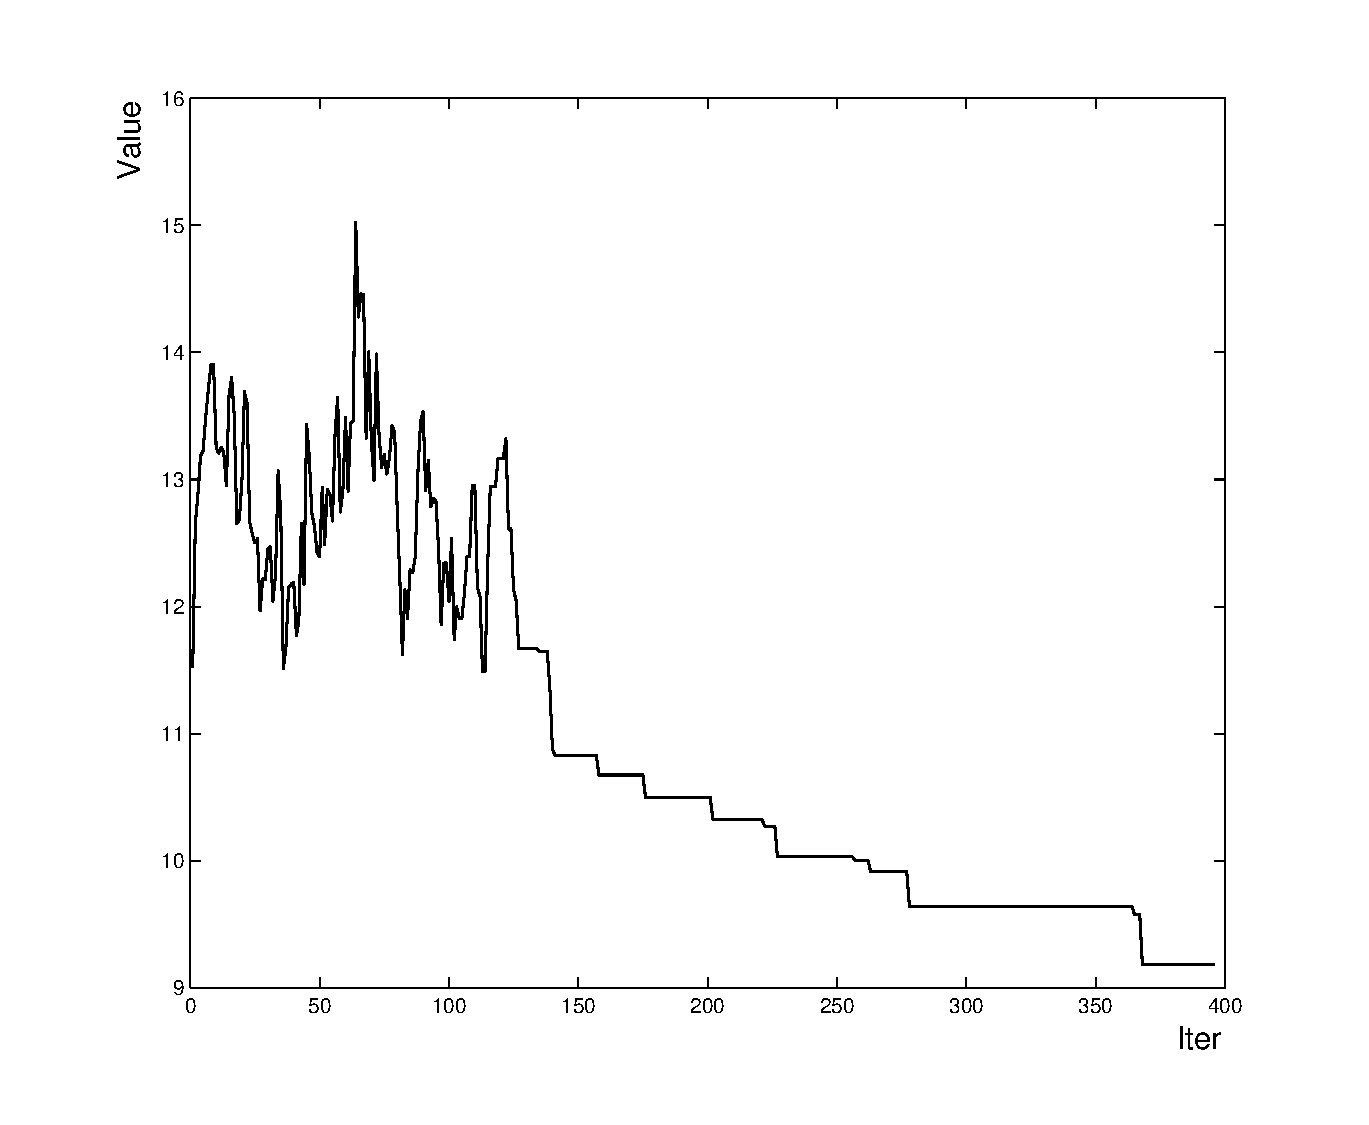
\includegraphics[width=0.8\textwidth]{figures/feasibility.eps}
\caption{算法收敛} \label{fig:feas}
\end{figure}
\section{稳定性}
我们已经看到算法可以成功收敛,但是如果每次收敛的结果差距过大则说明算法并不稳定,即不能保证每次都能得到一个较好的解。从下表\ref{tab:stability}我们可以看到,当取$N_v = 100, N_p = 100$时,十组不同数据的测试最终收敛的结果非常相近,并且都是较好的解。说明算法具有一定的稳定性,对初值并不敏感。

\begin{table}[htbp]
  \centering
  \small
  \begin{threeparttable}
    \caption{\label{tab:stability}算法稳定性}
    \begin{tabular}{cccccc}
      \toprule
        & 评价 & PM使用率 & RAM均衡负载 & CPU均衡负载 & 平均冲突率 \\
      \midrule
      1 & 4.019 & 0.760 & 0.184 & 0.270 & 1.061 \\
      2 & 3.692 & 0.770 & 0.241 & 0.180 & 1.110 \\
      3 & 4.643 & 0.810 & 0.210 & 0.256 & 1.064 \\
      4 & 4.052 & 0.740 & 0.271 & 0.174 & 1.165 \\
      5 & 4.126 & 0.730 & 0.254 & 0.214 & 1.039 \\
      6 & 4.360 & 0.740 & 0.245 & 0.222 & 1.081 \\
      7 & 3.609 & 0.810 & 0.165 & 0.266 & 1.012 \\
      8 & 3.145 & 0.790 & 0.166 & 0.240 & 1.000 \\
      9 & 4.433 & 0.770 & 0.220 & 0.251 & 1.045 \\
     10 & 3.442 & 0.770 & 0.194 & 0.230 & 1.000 \\
      \bottomrule
    \end{tabular}
    \tiny
    \begin{tablenotes}
    \item [1]$N_v = 100,N_p = 100$

    \item [2] Using Simulated Annealing Algorithm \ref{algo:SA}
    \end{tablenotes}
  \end{threeparttable}
\end{table}

\section{结果}
我们选取了$100$到$1000$步长为$100$的十组数据规模,分别使用模拟退火算法\ref{algo:SA}和\texttt{First-Fit}算法对同一组数据进行计算,并取10次不同数据的平均值得到了下表\ref{tab:result}:

\begin{table}[htbp]
  \centering
  \small
  \begin{threeparttable}
    \caption{\label{tab:result}测试数据}
    \begin{tabular}{ccccccc}
      \toprule
数据规模       & 方法 & 评价  & PM使用率 & RAM均衡负载 & CPU均衡负载 & 平均冲突率 \\
      \midrule
$ N_v = 100 $ & SA & 3.815 & 0.780 & 0.207 & 0.221 & 1.072 \\ 
              & FF & 3.636 & 0.600 & 0.321 & 0.157 & 1.199 \\ 
\hline 
$ N_v = 200 $ & SA & 4.138 & 0.770 & 0.230 & 0.220 & 1.061 \\ 
              & FF & 2.943 & 0.635 & 0.331 & 0.120 & 1.165 \\ 
\hline
$ N_v = 300 $ & SA & 4.370 & 0.773 & 0.245 & 0.212 & 1.087 \\ 
              & FF & 2.374 & 0.587 & 0.344 & 0.100 & 1.182 \\ 
\hline
$ N_v = 400 $ & SA & 5.061 & 0.785 & 0.239 & 0.249 & 1.082 \\
              & FF & 1.627 & 0.585 & 0.293 & 0.082 & 1.159 \\ 
\hline
$ N_v = 500 $ & SA & 4.768 & 0.792 & 0.236 & 0.234 & 1.090 \\ 
              & FF & 2.022 & 0.588 & 0.330 & 0.089 & 1.177 \\ 
\hline
$ N_v = 600 $ & SA & 4.824 & 0.797 & 0.236 & 0.235 & 1.095 \\
              & FF & 2.218 & 0.607 & 0.313 & 0.098 & 1.189 \\
\hline
$ N_v = 700 $ & SA & 5.673 & 0.801 & 0.249 & 0.259 & 1.101 \\
              & FF & 1.917 & 0.593 & 0.320 & 0.087 & 1.168 \\ 
\hline
$ N_v = 800 $ & SA & 5.411 & 0.814 & 0.239 & 0.253 & 1.097 \\ 
              & FF & 1.935 & 0.598 & 0.312 & 0.089 & 1.163 \\
\hline
$ N_v = 900 $ & SA & 5.392 & 0.793 & 0.246 & 0.251 & 1.101 \\ 
              & FF & 1.684 & 0.573 & 0.305 & 0.082 & 1.170 \\ 
\hline
$ N_v = 1000 $ & SA & 5.433 & 0.796 & 0.248 & 0.248 & 1.109 \\ 
               & FF & 1.713 & 0.584 & 0.318 & 0.078 & 1.180 \\

      \bottomrule
    \end{tabular}
  \end{threeparttable}
\end{table}

\section{结论}
从实验获得的数据\ref{tab:result}中我们可以得到以下结论。

\subsection*{模拟退火算法是有效的}

First-Fit算法已经被证明是解决背包问题的一个高效的算法,从得到数据中我们可以看到,我们设计的基于模拟退火算法得到的效果接近于FF得到的效果。甚至在某些指标上比如平均冲突率得到比FF得到的更好的效果。

\subsection*{First-Fit算法在减少PM的使用上有更好的效果}

从FF算法和SA算法在PM使用率这一指标的对比来看,FF算法有更好的效果,其平均使用率要低$20\%$所有,即每$100$个随机虚拟机请求,FF算法要比本文所使用的算法少使用$20$个左右的实体机。

产生的这样结果有两方面的因素:

\begin{enumerate}
\item FF算法可以认为是以使用PM的数量作为评价的贪心算法,因为算法总是试图将请求部署在已经使用的PM上,只有所有已使用的PM都无法满足请求,才会申请新的PM.
\item 本文所使用的算法的评价函数是综合考量四种不同因素的结果(四者的乘积),因此算法总趋向于综合更优的解。而PM使用率仅是其中的一项因素。
\end{enumerate}

\subsection*{模拟退火算法在处理RAM负载均衡效果较好,而在CPU负载均衡效果不如FF算法}
从获得数据\ref{tab:result}中我们看到,SA算法得到的解总是有较低的RAM负载均衡但CPU的均衡负载不如FF算法。

产生在这样结果原因主要是由于:
\begin{enumerate}
\item FF算法在判断当前VM能否部署在某个PM上时是依据约束条件\eqref{eq:con:4},即是否有足够的CPU核心剩余可以被分配,这就使得FF算法得到的解由CPU``饱和''的PM构成。如果$C^{~used}_j/C^T$均趋近于$1$则反而被认为更加``均衡''。
\item 同样的,本文所使用的算法受到评价函数中其他因素的影响,因此不会趋近于某一个因素更优的解。
\end{enumerate}

\subsection*{评价函数的重要性}
从得到的数据和上面的讨论可以看出,评价函数对本文所使用的算法的``优劣''有很大影响。但是,我们靠什么去评价一个解的优劣呢?显然不能以评价函数来评价---我们已经知道在评价函数下是好的了。因此,使用启发式算法来求解实际问题,应当是提出分析问题根据需求给出评价函数的模型,通过算法求解后代回问题观察是否在实际问题中理论上优的解真的有效,根据观察的结果不断的修正评价函数的模型才能获得理想的结果。

\section{结语}
本文提出了一种基于模拟退火算法求解数据中心中虚拟机资源配置问题的方法。实验结果表明,本文所述方法取得了良好的效果,并能根据所需条件的不同调整算法参数达到适应的目的。在本文中,对背景问题做了若干假设。如何在实际应用中通过修改模型取得良好的效果,达到更好的性能和效率,是接下来值得研究的内容。




